% -*- TeX-master: "main"; fill-column: 72 -*-

\newcommand{\CategoricalUnivariateDistribution}{\defRef{CategoricalUnivariateDistribution}{CategoricalUnivariateDistribution-class}}
\newcommand{\UnivariateDistribution}{\defRef{UnivariateDistribution}{UnivariateDistribution-class}}
\newcommand{\Category}{\defRef{Category}{Category-class}}
\newcommand{\ContinuousUnivariateDistribution}{\defRef{ContinuousUnivariateDistribution}{ContinuousUnivariateDistribution-class}}
\newcommand{\DiscreteUnivariateDistribution}{\defRef{DiscreteUnivariateDistribution}{DiscreteUnivariateDistribution-class}}
\newcommand{\ListOfCategories}{\defRef{ListOfCategories}{ListOfCategories-class}}
\newcommand{\MultivariateDistribution}{\defRef{MultivariateDistribution}{MultivariateDistribution-class}}
\newcommand{\ExternalDistribution}{\defRef{ExternalDistribution}{ExternalDistribution-class}}
\newcommand{\UncertBound}{\defRef{UncertBound}{UncertBound-class}}

\newcommand{\BetaDistribution}{\defRef{BetaDistribution}{BetaDistribution-class}}
\newcommand{\CauchyDistribution}{\defRef{CauchyDistribution}{CauchyDistribution-class}}
\newcommand{\ChiSquareDistribution}{\defRef{ChiSquareDistribution}{ChiSquareDistribution-class}}
\newcommand{\ExponentialDistribution}{\defRef{ExponentialDistribution}{ExponentialDistribution-class}}
\newcommand{\FDistribution}{\defRef{FDistribution}{FDistribution-class}}
\newcommand{\GammaDistribution}{\defRef{GammaDistribution}{GammaDistribution-class}}
\newcommand{\InverseGammaDistribution}{\defRef{InverseGammaDistribution}{InverseGammaDistribution-class}}
\newcommand{\LaplaceDistribution}{\defRef{LaplaceDistribution}{LaplaceDistribution-class}}
\newcommand{\LogNormalDistribution}{\defRef{LogNormalDistribution}{LogNormalDistribution-class}}
\newcommand{\LogisticDistribution}{\defRef{LogisticDistribution}{LogisticDistribution-class}}
\newcommand{\NormalDistribution}{\defRef{NormalDistribution}{NormalDistribution-class}}
\newcommand{\ParetoDistribution}{\defRef{ParetoDistribution}{ParetoDistribution-class}}
\newcommand{\RayleighDistribution}{\defRef{RayleighDistribution}{RayleighDistribution-class}}
\newcommand{\StudentTDistribution}{\defRef{StudentTDistribution}{StudentTDistribution-class}}
\newcommand{\UniformDistribution}{\defRef{UniformDistribution}{UniformDistribution-class}}
\newcommand{\WeibullDistribution}{\defRef{WeibullDistribution}{WeibullDistribution-class}}
\newcommand{\BinomialDistribution}{\defRef{BinomialDistribution}{BinomialDistribution-class}}
\newcommand{\GeometricDistribution}{\defRef{GeometricDistribution}{GeometricDistribution-class}}
\newcommand{\HypergeometricDistribution}{\defRef{HypergeometricDistribution}{HypergeometricDistribution-class}}
\newcommand{\NegativeBinomialDistribution}{\defRef{NegativeBinomialDistribution}{NegativeBinomialDistribution-class}}
\newcommand{\PoissonDistribution}{\defRef{PoissonDistribution}{PoissonDistribution-class}}
\newcommand{\BernoulliDistribution}{\defRef{BernoulliDistribution}{BernoulliDistribution-class}}
\newcommand{\CategoricalDistribution}{\defRef{CategoricalDistribution}{CategoricalDistribution-class}}


\subsection{The \class{Distribution} class}
\label{Distribution-class}
\label{distribution-class}

The \Distribution class is the abstract class from which all distributions are derived.  They are organized here in much the same way they were in \uncertml, by whether they are univariate or multivariate, and whether they are continuous, discrete, or categorical.  In addition, the \ExternalDistribution inherits from \Distribution, as a 'generic' distribution definition class that allows the user to define any distribution in an external ontology such as ProbOnto.

%When a \Distribution is encountered, its parent \FunctionDefinition is defined as sampling from the defined distribution, and returning that sample.  It may contain any number of \token{UncertIdRef} strings, each of which must correspond to an \token{UncertId} defined in a \DistribInput in the same function.

{\color{red} Lucian: \controversial When these distributions were originally defined, they were being used in extended \FunctionDefinition elements to define actual draws from the distributions.  Now that that part of the spec has been replaced by new csymbols, these distributions are now solely being used as children of the \Uncertainty element.  If people like this, great; if we want to ditch it for the \ExternalDistribution construct instead, that's fine.  We could even expand this list as some sort of automatic conversion of ProbOnto.}

In this draft of the \distrib specification, no mixed distributions and no multivariate distributions are presented, as the author has not seen any call for these distributions specifically, and believes that the generic \ExternalDistribution distribution could cover those cases on an as-needed basis.  If this turns out to not be the case, those distributions will be added to a subsequent version of this specification.  The use of the Arrays package would be required for any multivariate distribution.

The full list of distributions is included in \apdx{apdx-distributions}.

\subsubsection{Attributes inherited from \SBase}

A \Distribution always inherits the optional \token{metaid} and \token{sboTerm} attributes, and inherits optional \token{id} and \token{name} attributes as described in \sec{sec:idname}.  The \token{id} of a \Distribution has no mathematical meaning.


\subsection{The \class{UncertBound} class}
\label{UncertBound-class}
\label{uncertbound-class}

The \UncertBound class inherits from \UncertValue and adds a single required Boolean attribute \token{inclusive}.  This attribute indicates whether the value the bound represents is to be included in that range (\val{true}) or not (\val{false}).  This allows the creation of either ``open'' or ``closed'' boundaries of the ranges it is used to define.





\section{Distributions}
\label{apdx-distributions}

\subsection{The \class{UnivariateDistribution} class}
\label{UnivariateDistribution-class}
\label{univariatedistribution-class}

The \UnivariateDistribution class is an abstract class that derives from the \Distribution abstract class, and which has three derived classes itself: \ContinuousUnivariateDistribution, \DiscreteUnivariateDistribution, and \CategoricalUnivariateDistribution.  It is provided as a bookkeeping class to distinguish it from other types of distributions.


\subsection{The \class{MultivariateDistribution} class}
\label{MultivariateDistribution-class}
\label{multivariatedistribution-class}

The \MultivariateDistribution class is an abstract class with no derived classes in the current specification, but some could be added in the future.  Most likely, it will be removed from the final version of the spec.


\begin{figure}[htb]
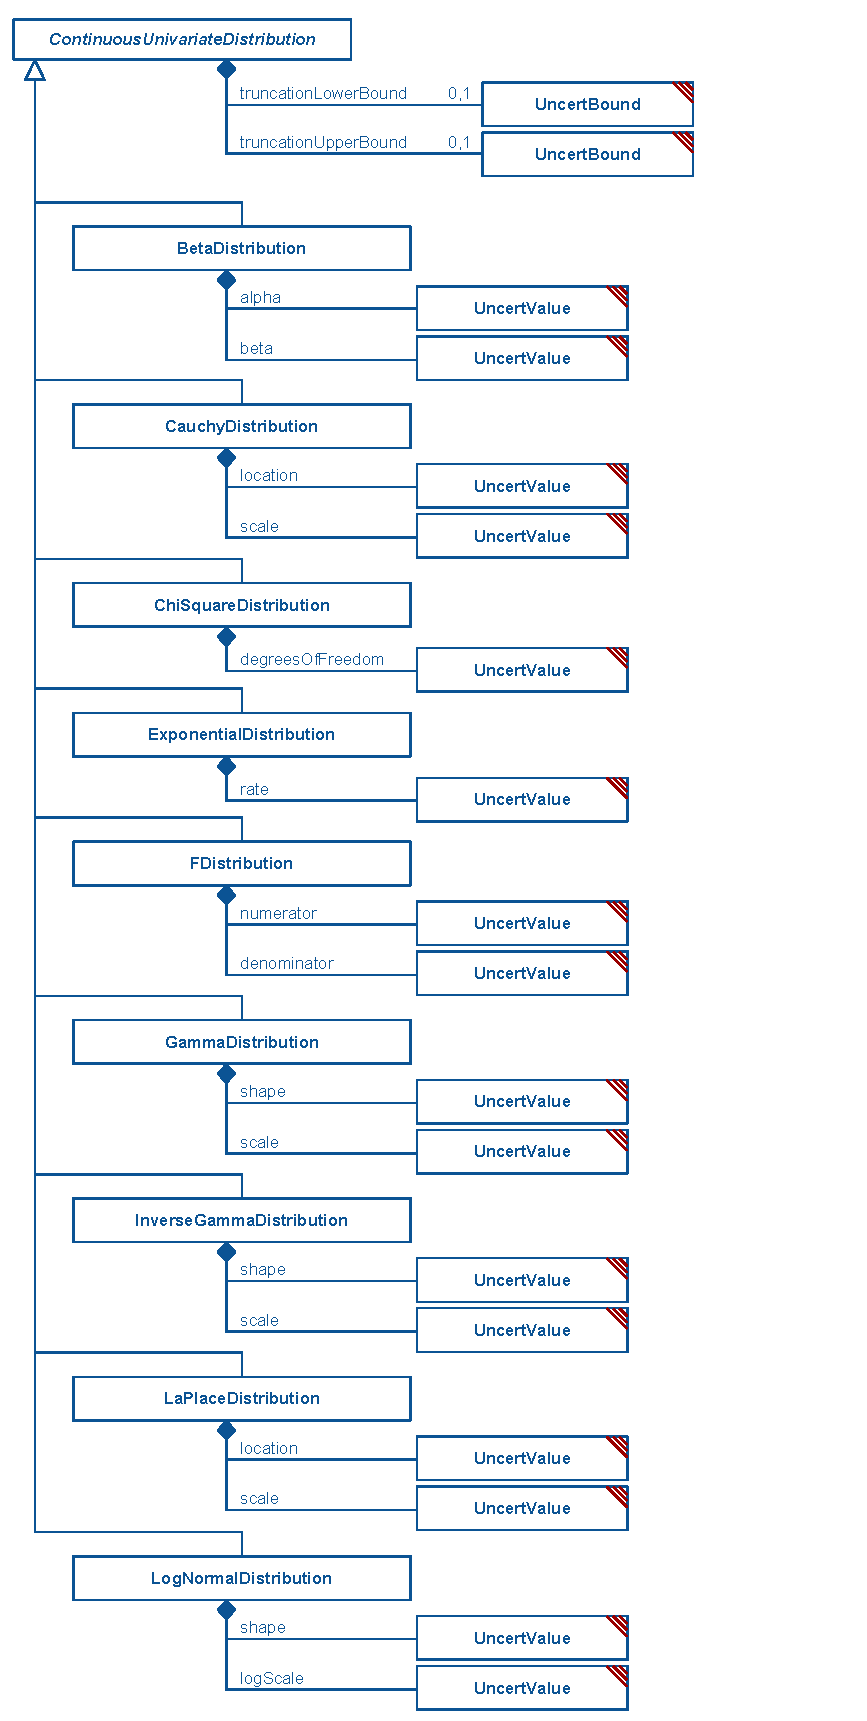
\includegraphics[width=0.6\linewidth]{figs/continuousUnivariateDistribution_first.pdf}
\caption{The definition of the \ContinuousUnivariateDistribution abstract class, and its \BetaDistribution, \CauchyDistribution, \ChiSquareDistribution, \ExponentialDistribution, \FDistribution, \GammaDistribution, \InverseGammaDistribution, \LaplaceDistribution, and \LogNormalDistribution children.  All may have lower and upper \UncertBound children, and each has one or more other parameters encoded as \UncertValue children (both defined below).}
\label{fig:continuousUnivariateDistribution_first}
\end{figure}


\subsection{The \class{ContinuousUnivariateDistribution} class}
\label{ContinuousUnivariateDistribution-class}
\label{continuousunivariatedistribution-class}
The abstract \ContinuousUnivariateDistribution class is the base class for a wide variety of distributions, all of which describe a potentially-bounded continuous range of probabilities.  Many of the most commonly-used distributions such as the \NormalDistribution and the \UniformDistribution fall into this category.

\begin{figure}[htb]
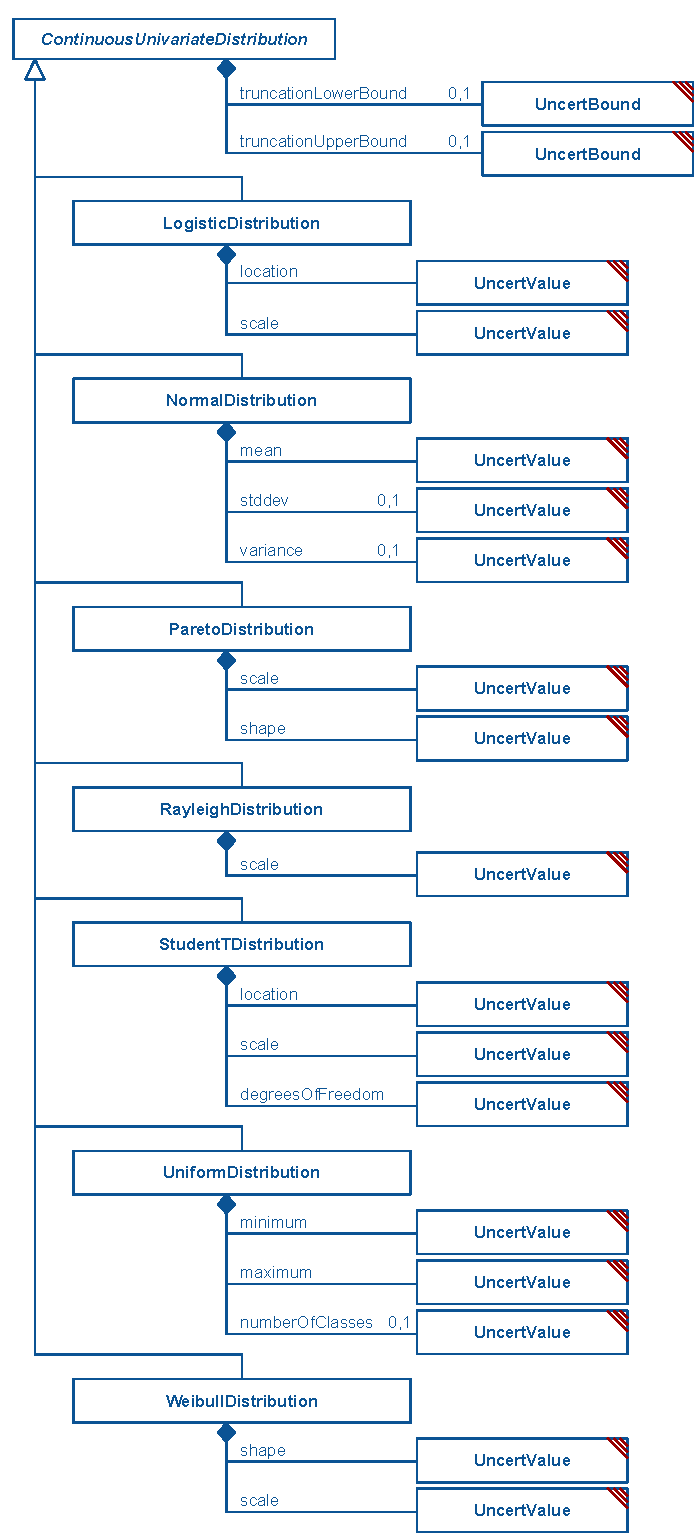
\includegraphics[width=0.55\linewidth]{figs/continuousUnivariateDistribution_second.pdf}
\caption{The definition of the \ContinuousUnivariateDistribution abstract class, and its \LogisticDistribution, \NormalDistribution, \ParetoDistribution, \RayleighDistribution, \StudentTDistribution, \UniformDistribution, and \WeibullDistribution children.  All may have lower and upper \UncertBound children, and each has one or more other parameters encoded as \UncertValue children (both defined below).}
\label{fig:continuousUnivariateDistribution_second}
\end{figure}

All \ContinuousUnivariateDistribution elements may have two optional children: \val{lowerTruncationBound} and \val{upperTruncationBound}, both of the class \UncertBound (defined below).  Either element, if present, limit the range of possible sampled values from the distribution.  The \val{lowerTruncationBound} defines the lowest value (inclusive or not, as defined by that element's \token{inclusive} attribute) that can be sampled, and the \val{upperTruncationBound} defines the highest.  If both children are present, the \val{lowerTruncationBound} must either be lower than the \val{upperTruncationBound}, or they may be equal, if both bounds are set \token{inclusive}=\val{true}.  Similarly, some distributions are themselves naturally bound (some may, for example, only return values greater than zero).  In those cases, the natural lower bound of the distribution must either be lower than the \val{upperTruncationBound}, or be equal to it if the natural lower bound is inclusive, and if the \val{upperTruncationBound} is set \token{inclusive}=\val{true}.  Similarly, the natural upper bound of the distribution must either be higher than the \val{lowerTruncationBound}, or it may be equal to it if the natural upper bound is inclusive and if the \val{lowerTruncationBound} is set \token{inclusive}=\val{true}.  It may be impossible to determine this from a static analysis of the model, as either or both bound's values may depend on other dynamic variables.  If a simulator encounters this situation, the sampled value and the behavior of the simulator are undefined.

If bounded, the cumulative probability that would have been assigned to the region outside the bound is re-assigned proportionally to the rest of the distribution.  It should be noted that while discarding any value obtained from the non-truncated version of the distribution and re-sampling is indeed one method that could be used to accomplish this, the efficiency of that algorithm decreases with the width of the allowed window, and indeed is technically zero (and would take an infinite amount of time to complete) should the bounds be equal to one another.  Taking any samples obtained outside the bound window and instead returning the boundary value itself is incorrect, and will not result in a proper draw from the defined distribution.

The distributions of this type allowed in this version of the specification are defined in \fig{fig:continuousUnivariateDistribution_first} and \fig{fig:continuousUnivariateDistribution_second}.  A full list of all of the distributions is provided in \sec{sec:allDistributions}.


\begin{figure}[htb]
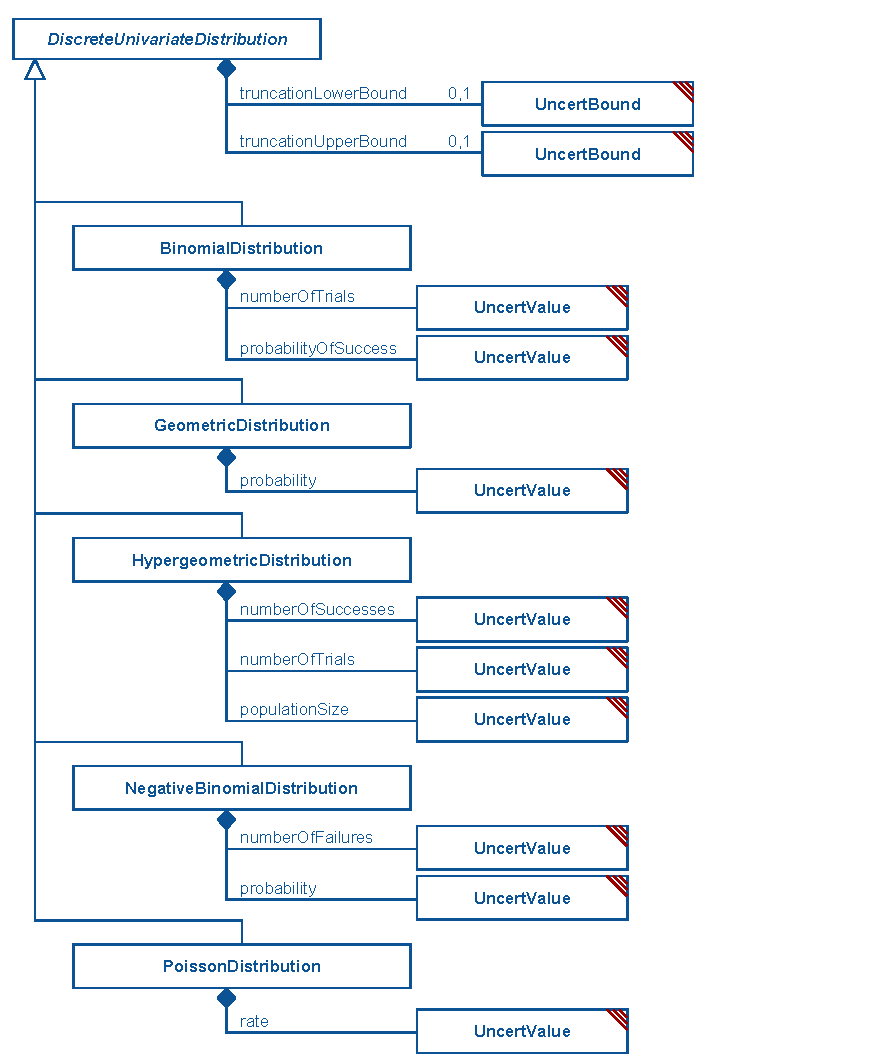
\includegraphics[width=0.7\linewidth]{figs/discreteUnivariateDistribution.pdf}
\caption{The definition of the \DiscreteUnivariateDistribution abstract class, and its \BinomialDistribution, \GeometricDistribution, \HypergeometricDistribution, \NegativeBinomialDistribution, and \PoissonDistribution children.  All may have lower and upper \UncertBound children, and each has one or more other parameters encoded as \UncertValue children (both defined below).}
\label{fig:discreteUnivariateDistribution}
\end{figure}

\subsection{The \class{DiscreteUnivariateDistribution} class}
\label{DiscreteUnivariateDistribution-class}
\label{discreteunivariatedistribution-class}

The abstract \DiscreteUnivariateDistribution class is the base class for a wide variety of distributions, all of which describe a potentially-bounded range of probabilities of discrete values.  The most commonly-used distributions in this class is probably the \PoissonDistribution.  Distributions that always return integers fall in this category, which often involve events happening at particular frequencies.

All \DiscreteUnivariateDistribution elements (like \ContinuousUnivariateDistribution elements) may have two optional children: \val{lowerTruncationBound} and \val{upperTruncationBound}, both of the class \UncertBound (defined below).  Either element, if present, limit the range of possible sampled values from the distribution.  The \val{lowerTruncationBound} defines the value below which no sampling may take place
(inclusive or not, as defined by that element's \token{inclusive} attribute), and the \val{upperTruncationBound} defines the value above which no sampling may take place.  These bounds may fall between the possible discrete values being returned:  as an example, for a distribution that returned an integer in the series [0, 1, 2, ...], if it was given a \val{lowerTruncationBound} of 1.5, the lowest value it could return would be 2.  In this case, the value of the \token{inclusive} attribute on the \UncertBound would be immaterial, as '1.5' could never be returned.

As \changed{with} \ContinuousUnivariateDistribution bounds, if both bounds are present, the \val{lowerTruncationBound} must either be lower than the \val{upperTruncationBound}, or they may be equal, if both bounds are set \token{inclusive}=\val{true}.  Similarly, the discrete distributions are themselves often naturally bound (some may, for example, only return values greater than zero).  In those cases, the natural lower bound of the distribution must be either be lower than the \val{upperTruncationBound}, or it may be equal to it if the natural lower bound is inclusive, and if the \val{upperTruncationBound} is set \token{inclusive}=\val{true}.  Similarly, the natural upper bound of the distribution must either be higher than the \val{lowerTruncationBound}, or it may be equal to it if the natural upper bound is inclusive and if the \val{lowerTruncationBound} is set \token{inclusive}=\val{true}.  In addition, if both bounds are defined, they must define a span within which at least one possible sampled discrete value may be found.  For a distribution that returns integers, for example, one may not define a lower bound of 1.5 and an upper bound of 1.8, as no integer lies within that range.  It may be impossible to determine if any of these rules are violated from a static analysis of the model, as either or both bound's values may depend on other dynamic variables.  If a simulator encounters this situation, the sampled value and the behavior of the simulator are undefined.

If bounded, the cumulative probability that would have been assigned to the values outside the bound is re-assigned proportionally to the rest of the distribution.  It should be noted that while discarding any value obtained from the non-truncated version of the distribution and re-sampling is indeed one method that could be used to accomplish this, the efficiency of that algorithm decreases with the width of the allowed window, and indeed is technically zero (and could take an infinite amount of time to complete) should the bounds allow only a single discrete value.  Taking any samples obtained outside the bound window and instead returning the boundary value itself is incorrect, and will not result in a proper draw from the defined distribution.

The distributions of this type allowed in this version of the specification are defined in \fig{fig:discreteUnivariateDistribution}.  A full list of all of the distributions is provided in \sec{sec:allDistributions}.



\begin{figure}[htb]
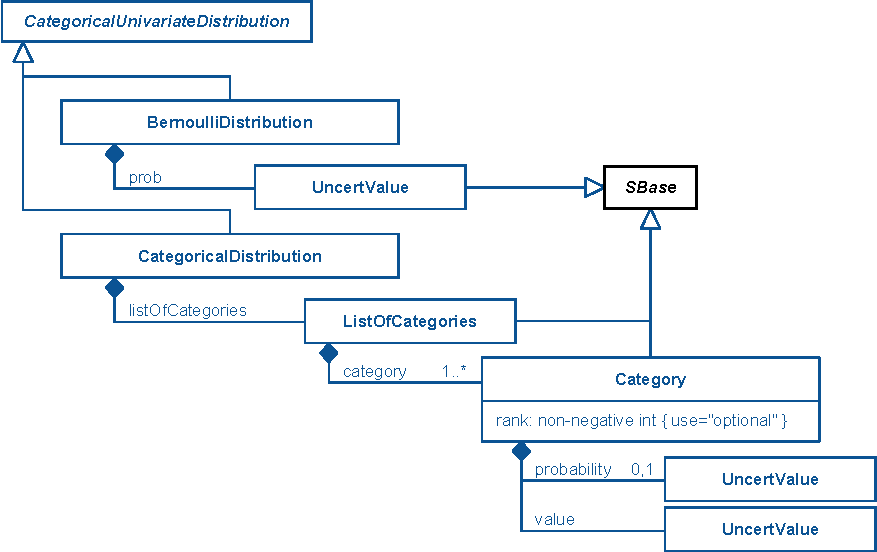
\includegraphics[width=0.8\linewidth]{figs/categoricalUnivariateDistribution.pdf}
\caption{The definition of the \CategoricalUnivariateDistribution abstract class, plus the \BernoulliDistribution, \CategoricalDistribution, \ListOfCategories, and \Category classes.}
\label{fig:categoricalUnivariateDistribution}
\end{figure}

\subsection{The \class{CategoricalUnivariateDistribution} class}
\label{CategoricalUnivariateDistribution-class}
\label{categoricalunivariatedistribution-class}

The \CategoricalUnivariateDistribution abstract class includes distributions where the various possible sampled values are each explicitly listed, along with the probability for that sampled value.  The sum of these probabilities must therefore equal 1.0, in order to be valid.  This type of distribution class is used for things such as weighted die rolls, or other situations where particular values are obtained at arbitrary probabilities.

Because each possible sampled value is explicitly listed in an \CategoricalUnivariateDistribution, it does not have the optional \UncertBound values that the other univariate distributions do: if a particular value is not allowed, it is simply dropped from the list of options, and the probabilities of the other values are scaled accordingly.


\begin{figure}[htb]
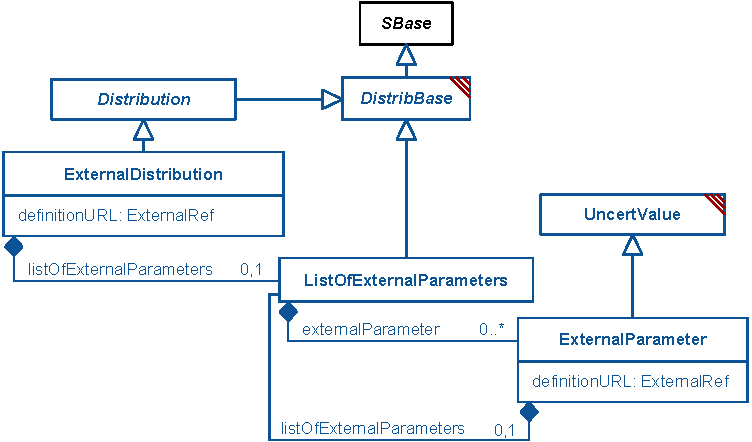
\includegraphics[width=0.5\linewidth]{figs/externalDistribution.pdf}
\caption{The definition of the \ExternalDistribution, \ExternalParameter, and \ListOfExternalParameters classes.  These classes define a way to define a distribution with reference to an external database or ontology of distribution definitions.}
\label{fig:externalDistribution}
\end{figure}

\subsection{The \class{ExternalDistribution} class}
\label{ExternalDistribution-class}
\label{externaldistribution-class}

The \ExternalDistribution class is provided to allow a modeler to encode a distribution not otherwise explicitly handled by this specification.  Because the range of possibilities is so vast, the modeler should not normally expect any given SBML simulator or other software to be able to properly manipulate this distribution, but particular software tools may implement support for certain distributions they know their own software's users may require.

The required attribute \token{definitionURL}, of type \primtype{ExternalRef}, must be a URI that defines a valid distribution.  It is strongly recommended that modelers use distributions from ProbOnto (\url{http://probonto.org/}), as consistently referencing a single ontology will improve exchangeability, at least slightly.  The referenced distribution is then the distribution defined by this \ExternalDistribution, along with any parameterization provided by the children \ExternalParameter elements.

Some referenced distributions are multivarite, meaning they define correlated distributions for two or more parameters.  It is impossible with \sbmlthreecore to define a \FunctionDefinition that returns a vector, and similarly no \primtype{SId} in \sbmlthreecore can be used to represent a vector.  If this is desired, then, the Arrays package must be used in concert with the \ExternalDistribution to cooperatively set up a model with a \FunctionDefinition that can use an array as input and/or as output.

The \ExternalDistribution defines an optional child \ListOfExternalParameters, which can be used to parameterize the defined distribution.


\subsection{Specific Distributions}
\label{sec:allDistributions}

In this table, all distributions are listed, along with their types (Continuous, Categorical, or Discrete), whether they're univariate or multivariate, and a brief description.  The element name is the name of the distribution with spaces removed, the initial letter lower-cased, and \val{Distribution} appended, so, for example, the \val{Exponential} distribution becomes \val{<exponentialDistribution>}, and the \val{Student T} distribution becomes \val{<studentTDistribution>}.
%The exception is that all of the mixture models (ones that end with \val{Mixture Model}), only have spaces removed but nothing appended:  the Continuous Univariate Mixture Model becomes \val{<ContinuousUnivariateMixtureModel>}, etc.

All of these distributions inherit from the abstract \Distribution class.  Additionally, the appropriate distributions inherit from the \UnivariateDistribution or \MultivariateDistribution abstract classes, and further from the \ContinuousUnivariateDistribution, \DiscreteUnivariateDistribution, or \CategoricalUnivariateDistribution classes, which are related to one another as one would expect.

All descriptions are based on the information from \url{http://www.uncertml.org/}, which is now defunct, but which can still be accessed at \url{http://web.archive.org/web/20160313012501/uncertml.org}.

Distributions are listed grouped by category (type and univarite/multivariate), and alphabetical within those categories.


\subsection{The \class{BetaDistribution} class}
\label{BetaDistribution-class}
\label{betadistribution-class}

The \BetaDistribution is a \ContinuousUnivariateDistribution that defines the \UncertValue children \token{alpha} ($\alpha$) and \token{beta} ($\beta$).  Both \token{alpha} and \token{beta} must be positive.

A random variable x is Beta distributed if the probability density function (pdf) is of the form:

\begin{center}
$\dfrac{1}{B\left(\alpha,\beta\right)}x^{\alpha-1}\left(1-x\right)^{\beta-1}$, where $B\left(\alpha,\beta\right)$ = $\dfrac{\Gamma\left(\alpha\right)\Gamma\left(\beta\right)}{\Gamma\left(\alpha+\beta\right)}$
\end{center}

The distribution is usually denoted as $x\sim Be\left(\alpha,\beta\right)$ with parameters $\alpha$ and $\beta$, both positive real values. As the domain of the random variable is defined to be $[0,1]$ the Beta distribution is normally used to describe the distribution of a probability value.

\subsection{The \class{CauchyDistribution} class}
\label{CauchyDistribution-class}
\label{cauchydistribution-class}

The \CauchyDistribution is a \ContinuousUnivariateDistribution that defines the \UncertValue children \token{location} ($\theta$) and \token{scale} ($\gamma$).  The \token{scale} value must be positive.

A random variable x follows a Cauchy distribution if the probability density function (pdf) is of the form:

\begin{center}
$\dfrac{1}{\pi\gamma}\left[1+\left(\dfrac{x-\theta}{\gamma}\right)^2\right]^{-1}$
\end{center}

The Cauchy distribution is equivalent to a Student-T distribution with 1 degree of freedom. It is widely used in physics, optics and astronomy. It is also known as the Lorenz or the Breit-Wigner distribution.

\subsection{The \class{ChiSquareDistribution} class}
\label{ChiSquareDistribution-class}
\label{chisquaredistribution-class}

The \ChiSquareDistribution is a \ContinuousUnivariateDistribution defining a \UncertValue child \token{degreesOfFreedom} ($\nu$).  The \token{degreesOfFreedom} must be a positive integer.

A random variable x is Chi-square distributed if the probability density function (pdf) is of the form:

\begin{center}
$\dfrac{1}{\Gamma(\nu/2)2^{\nu/2}}x^{\nu/2-1}exp(-x/2)$
\end{center}

The distribution is usually denoted as $x\sim\chi_\nu$ where $\nu$ is known as the degrees of freedom parameter. $\nu$ has to be positive and $x$ has to be non-negative for the density to be defined. The Chi-square distribution is a special case of the Gamma distribution where $\chi \sim\Gamma(k=\nu/2,\theta=2)$.

\subsection{The \class{ExponentialDistribution} class}
\label{ExponentialDistribution-class}
\label{exponentialdistribution-class}

The \ExponentialDistribution is a \ContinuousUnivariateDistribution that defines the \UncertValue child \token{rate} ($\lambda$).  The \token{rate} value must be positive.

A random variable x follows an exponential distribution if the probability density function (pdf) is of the form:

\begin{center}
$\lambda e^{-\lambda x}$
\end{center}

It is often represented as $x \sim$ Exp$(\lambda)$. It is used to model the time between events for a Poisson process and is used in simulation of stochastic systems.

\subsection{The \class{FDistribution} class}
\label{FDistribution-class}
\label{fdistribution-class}

The \FDistribution is a \ContinuousUnivariateDistribution that defines the \UncertValue children \token{numerator} ($\nu_1$) and \token{denominator} ($\nu_2$).  Both \token{numerator} and \token{denominator} must be positive integers.

A random variable x follows an F distribution if the probability density function (pdf) is of the form:

\begin{center}
$\dfrac{ 1 } {B(\nu_1/2, \nu_2/2)} \left( \dfrac{\nu_1}{\nu_2}\right)^{\nu_1/2} x^{\nu_1/2 - 1} \left(1 + \dfrac{\nu_1}{\nu_2}x \right)^{-\frac{\nu_1+\nu_2}{2} }$
\end{center}

where $B(.)$ is the Beta function. It often arises as the ratio of two random variables that are identically Chi-Square distributed.

\subsection{The \class{GammaDistribution} class}
\label{GammaDistribution-class}
\label{gammadistribution-class}

The \GammaDistribution is a \ContinuousUnivariateDistribution that defines the \UncertValue children \token{shape} ($k$) and \token{scale} ($\theta$).  Both \token{shape} and \token{scale} must be positive.

A random variable x is Gamma distributed if the probability density function (pdf) is of the form:

\begin{center}
$\dfrac{1}{\Gamma(k) \theta^k} x^{k-1} exp(-x/\theta) $ with $ \Gamma(\cdot) $ the Gamma function.
\end{center}

The distribution is usually denoted as $x \sim Gamma(k, \theta)$ where $k$ is known as the shape parameter and $\theta$ the scale parameter. Both parameters have be positive and $x$ has to be non-negative for the density to be defined. In practice the Gamma distribution is often use to model the distribution of non-negative quantities such as variances.

\subsection{The \class{InverseGammaDistribution} class}
\label{InverseGammaDistribution-class}
\label{inversegammadistribution-class}

The \InverseGammaDistribution is a \ContinuousUnivariateDistribution that defines the \UncertValue children \token{shape} ($\alpha$) and \token{scale} ($\beta$).  Both \token{alpha} and \token{beta} must be positive.

A random variable x is Inverse Gamma distributed if the probability density function (pdf) is of the form:

\begin{center}
$\dfrac{\beta^\alpha}{\Gamma(\alpha)}x^{-\alpha-1}exp(-\beta/x)$
\end{center}

If variable $x$ is Inverse Gamma distributed, 1/$x$ is gamma distributed. The Inverse Gamma distribution function can be obtained from the Gamma distribution by a transformation of variables.

\subsection{The \class{LaplaceDistribution} class}
\label{LaplaceDistribution-class}
\label{laplacedistribution-class}

The \LaplaceDistribution is a \ContinuousUnivariateDistribution that defines the \UncertValue children \token{location} ($\mu$) and \token{scale} ($b$).  The \token{scale} value must be positive.

A random variable x is Laplace distributed if the probability density function (pdf) is of the form:

\begin{center}
$\dfrac{1}{2b}\mathrm{exp}\bigg(-\dfrac{abs(x-\mu)}{b}\bigg)$
\end{center}

where $abs$ denotes the absolute value. It can be thought of as a combination of two exponential distributions.

\subsection{The \class{LogNormalDistribution} class}
\label{LogNormalDistribution-class}
\label{lognormaldistribution-class}

The \LogNormalDistribution is a \ContinuousUnivariateDistribution that defines the \UncertValue children \token{shape} ($\sigma^2$) and \token{logScale} ($\mu$).  The \token{shape} value must be positive.

A random variable x is Log Normal distributed if the probability density function (pdf) is of the form:

\begin{center}
$\dfrac{1}{x \sqrt{2 \pi \sigma^2}} \mathrm{exp}\bigg(-\dfrac{ (\mathrm{ln}(x)-\mu)^2 }{2 \sigma^2}\bigg)$
\end{center}

If variable x is normally distributed, exp(x) is Log Normal distributed. The Log Normal distribution function can be obtained from the normal distribution by a transformation of variables. It is often used for variables that must be positive.

\subsection{The \class{LogisticDistribution} class}
\label{LogisticDistribution-class}
\label{logisticdistribution-class}

The \LogisticDistribution is a \ContinuousUnivariateDistribution that defines the \UncertValue children \token{location} ($\mu$) and \token{scale} ($s$).  The \token{scale} value must be positive.

A random variable x is Logistic distributed if the probability density function (pdf) is of the form:

\begin{center}
$\dfrac{\mathrm{exp}(-(x-\mu)/s)}{s(1+\mathrm{exp}\big(-(x-\mu)/s)\big)^2}$
\end{center}

\subsection{The \class{NormalDistribution} class}
\label{NormalDistribution-class}
\label{normaldistribution-class}

The \NormalDistribution is a \ContinuousUnivariateDistribution that defines the \UncertValue children \token{mean} ($\mu$), \token{stddev} ($\sigma$), and \token{variance} ($\sigma^2$).  The distribution must either define a \token{stddev} or a \token{variance}, but not both.  The \token{variance}, if defined, must be positive.

A random variable x is normally distributed if the probability density function (pdf) is of the form:

\begin{center}
$\dfrac{1}{\sqrt{2\pi\sigma^2}}\mathrm{exp}\big(-\frac{(x-\mu)^2}{2\sigma^2}\big)$
\end{center}

The distribution is usually denoted as $x\sim \mathcal{N}(\mu,\sigma^2)$ where $\mu$ is known as the mean parameter and $\sigma^2$ the variance parameter. If the random variable x is a vector of length greater than one, the normal distribution can be generalised to the Multivariate normal.  A reason for the widespread usage of the normal distribution is the Central limit theorem which states that the distribution of the mean of a large number of independent identically distributed random variables tends to a normal distributions as the number of random variables increases.

\subsection{The \class{ParetoDistribution} class}
\label{ParetoDistribution-class}
\label{paretodistribution-class}

The \ParetoDistribution is a \ContinuousUnivariateDistribution that defines the \UncertValue children \token{scale} ($x_m$) and \token{shape} ($\alpha$).  Both \token{shape} and \token{scale} must be positive.

A random variable x follows a Pareto distribution if the probability density function is of the form:

\begin{center}
$\dfrac{\alpha x_m^\alpha}{x^{\alpha+1}}$
\end{center}

The distribution allows for the specification of a minimum value below which the density is 0. It is a skewed heavy-tailed distribution.

\subsection{The \class{RayleighDistribution} class}
\label{RayleighDistribution-class}
\label{rayleighdistribution-class}

The \RayleighDistribution is a \ContinuousUnivariateDistribution that defines the \UncertValue children \token{scale}.

[From Wikipedia:] A Rayleigh distribution is often observed when the overall magnitude of a vector is related to its directional components. One example where the Rayleigh distribution naturally arises is when wind velocity is analyzed into its orthogonal 2-dimensional vector components. Assuming that each component is uncorrelated, normally distributed with equal variance, and zero mean, then the overall wind speed (vector magnitude) will be characterized by a Rayleigh distribution. A second example of the distribution arises in the case of random complex numbers whose real and imaginary components are independently and identically distributed Gaussian with equal variance and zero mean. In that case, the absolute value of the complex number is Rayleigh-distributed.

\subsection{The \class{StudentTDistribution} class}
\label{StudentTDistribution-class}
\label{studenttdistribution-class}

The \StudentTDistribution is a \ContinuousUnivariateDistribution that defines the \UncertValue children  \token{location} ($\mu$), \token{scale} ($\sigma^2$) and \token{degreesOfFreedom} ($\nu$).

A random variable x follows a Student-t distribution if the probability density function (pdf) is of the form:

\begin{center}
$\dfrac{\Gamma(\nu/2+1/2)}{\Gamma(\nu/2)(\pi\nu\sigma^2)^{1/2}}\big[1+\frac{(x-\mu)^2}{\nu\sigma^2}\big]^{-\nu/2-1/2}$. The distribution is usually denoted as $x\sim St(\mu,\lambda,\nu)$
\end{center}

This distribution corresponds to integrating out the variance of a normal distribution using a inverse Gamma prior. It can therefore be interpreted as an infinite mixture of normal distributions having the same mean but different variances. The three parameters are the mean ($\mu$), degrees of freedom ($\nu$) and variance ($\sigma^2$). Setting the variance to 1 and the mean to 0 we obtain the Student-t form found in standard statistics references such as Wikipedia. Setting the d.f. to 1 the Cauchy distribution is obtained. Setting the d.f. to infinity the normal distribution is obtained. The student-t distribution is commonly used in likelihood inference as the maximum likelihood parameter estimates are more robust to outlier observations compared to the normal distribution.

\subsection{The \class{UniformDistribution} class}
\label{UniformDistribution-class}
\label{uniformdistribution-class}

The \UniformDistribution is a \ContinuousUnivariateDistribution that defines the \UncertValue children \token{minimum} ($a$), \token{maximum} ($b$) and the optional \token{numberOfClasses}.  The \token{minimum} value must be less than the \token{maximum} value.  If \token{numberOfClasses} is defined, its value must be an integer greater than or equal to two.

A random variable x follows a uniform distribution if the probability density function (pdf) is of the form:

\begin{center}
$\dfrac{1}{b-a}$
\end{center}

The distribution assigns equal probability to all events within the chosen domain between (and including) the minimum ($a$) and the maximum ($b$).

If \token{numberOfClasses} is included, the uniform range is divided into $numberOfClasses-1$ sections, and each of the borders of those sections are equally likely to be returned.  If \token{numberOfClasses} is 2 (the minimum), the range just has $2-1=1$ section, and the borders of that section (the \token{minimum} and \token{maximum}) are the two possible return values.  If \token{numberofClasses} is 3, the range is broken into $3-1=2$ sections, leaving the \token{minimum}, \token{maximum}, and mean as the three possible return values, etc.

\subsection{The \class{WeibullDistribution} class}
\label{WeibullDistribution-class}
\label{weibulldistribution-class}

The \WeibullDistribution is a \ContinuousUnivariateDistribution that defines the \UncertValue children \token{shape} ($k$) and \token{scale} ($\lambda$).  Both \token{shape} and \token{scale} must be positive.

A random variable x follows an Weibull distribution if the probability density function (pdf) is of the form:

\begin{center}
$\dfrac{k}{\lambda}\left(\dfrac{x}{\lambda}\right)^{k-1}\mathrm{exp}\bigg(\dfrac{-x}{\lambda}\bigg)^k$
\end{center}

It includes the exponential distribution as a special case. It is often used in engineering and finance.

%Continuous Multivariate Mixture Model & Continuous & Multivariate 
%  & A mixture model is a linear combination of base distributions. A widely used case is where the base distributions are Gaussian in which case the model is known as the Gaussian Mixture Model.
%Dirichlet & Continuous & Multivariate 
%  & A $K$ dimensional random variable x follows a Dirichlet distribution if the probability density function (pdf) is of the form $\frac{1}{B(\mathbf{a})} \prod_{i=1}^K x_i^{\alpha_i - 1}$ where $B(\mathbf{a}) = \frac{ \prod^k_{i=1} \Gamma(\alpha_i) } { \Gamma( \sum_{i=1}^K \alpha_i ) }$ and $\Gamma(.)$ is the Gamma function. It is the multivariate extension of the beta distribution to higher dimensions with K a positive integer greater than or equal to 2.
%Multivariate Normal & Continuous & Multivariate 
%  & The Multivariate Normal is an extension of the univariate normal distribution to higher dimensional vector spaces. A random vector variable of dimension $ k $  denoted $ \mathbf{x} $ is normally distributed if the probability density function (pdf) is of the form $(2 \pi)^{-k/2} \mathrm{det}(\Sigma)^{-1/2} exp (-\frac{1}{2} (\mathbf{x} - \mathbf{\mu})^T \Sigma^{-1} (\mathbf{x} - \mathbf{\mu}) ) $ where $ \mathrm{det}(.) $ denotes the determinant and $ (.)^T $ the matrix transpose. The distribution is usually denoted as $ \mathbf{x} \sim \mathcal{N}(\mathbf{\mu}, \Sigma) $ where $ \mathbf{\mu} $ is known as the mean vector parameter and $ \Sigma $ the covariance matrix parameter.
%Multivariate Student T & Continuous & Multivariate 
%  & A random variable $ \mathbf{x} $ follows a multivariate Student-t distribution if the probability density function (pdf) is of the form $\frac{ \Gamma(\nu/2 + k/2)} {\Gamma(\nu/2) (\pi \nu)^{k/2} \mathrm{det} (\Sigma)^{1/2} } \left[1 + \frac{ \Delta^2 } { \nu } \right]^{-\nu/2 - k/2}  $ where $ \Delta^2 = (\mathbf{x} - \mathbf{\mu})^T \Sigma^{-1}  (\mathbf{x} - \mathbf{\mu}) $ is the squared Mahalanobis distance. The distribution is usually denoted as $ x \sim St(\mathbf{\mu},\Sigma,\nu) $. It is the extension of the univariate student-t distribution to higher dimensions. Student-t distributions are often used when tails are expected to be heavier than Gaussian or Normal, and can result from applying Bayesian inference.
%Normal Inverse Gamma & Continuous & Multivariate 
%  & A Normal Inverse Gamma distribution is the conjugate prior of a normal distribution with unknown mean and variance. It is the coupled product of an Inverse Gamma distribution and a normal distribution. In particular if $p(\mathbf{X} ; \mu, \sigma^2) $ is the likelihood function of a Normally distributed set of random variables with mean $ \mu $ and variance $ \sigma^2 $ and if both the mean and variance are considered unknown, the conjugate prior is $  p(\mu,\sigma^2) = p(\mu ; \sigma^2) p(\sigma^2) $ where $  p(\mu ; \sigma^2) = \mathcal{N}(\mu ; \mu_0, \sigma^2/\nu) $ a Normal prior on the mean and $ p(\sigma^2) = \mathrm{IG}(\sigma^2 ; \alpha, \beta) $ an Inverse Gamma prior on the variance. Note that the priors are not independent as the prior variance of the mean is a linear function of of the variance $ \sigma^2 $. It is also common to use a Normal-Gamma distribution where a conjugate prior is placed on the unknown mean and precision (i.e. inverse variance) of the Normal likelihood in which case the prior is a product of a Normal and Gamma distributions. In the case of a Multivariate normal likelihood, the corresponding conjugate prior is a Normal-Wishart distribution.

\subsection{The \class{BinomialDistribution} class}
\label{BinomialDistribution-class}
\label{binomialdistribution-class}

The \BinomialDistribution is a \DiscreteUnivariateDistribution that defines the \UncertValue children \token{numberOfTrials} ($n$) and \token{probabilityOfSuccess} ($\theta$).  The \token{numberOfTrials} must be a positive integer, and \token{probabilityOfSuccess} must be a value between zero and one, inclusive.

A random variable $ x $ follows a Binomial distribution if the probability mass function (pmf) is of the form:

\begin{center}
${n \choose x} \theta^x (1-\theta)^{n-x} $
\end{center}

where $ {n \choose x} $ denotes $ n $ choose $ x $. The distribution is usually denoted as $ x \sim b(n,\theta) $. The distribution describes the probability of getting $ x $ successes in $n$ trials of independent experiments that have the same probability of success.

\subsection{The \class{GeometricDistribution} class}
\label{GeometricDistribution-class}
\label{geometricdistribution-class}

The \GeometricDistribution is a \DiscreteUnivariateDistribution that defines the \UncertValue child \token{probability} ($p$).  The \token{probability} must have a value must be between zero and one, inclusive.

A random variable $ x $ follows a geometric distribution if the probability mass function (pmf) is of the form:

\begin{center}
$(1-p)^{x-1} p$
\end{center}

It is often represented as $x \sim \mathrm{Geom}(p)$. It is the discrete analogue of the exponential distribution. It is used to model distribution of the number of binary (Bernoulli) trials needed to get one success, with parameter, probability $p$.

\subsection{The \class{HypergeometricDistribution} class}
\label{HypergeometricDistribution-class}
\label{hypergeometricdistribution-class}

The \HypergeometricDistribution is a \DiscreteUnivariateDistribution that defines the \UncertValue children \token{numberOfSuccesses} ($m$). \token{numberOfTrials} ($n$), and \token{populationSize} ($N$).  All three values must be positive integers, chosen such that \token{numberOfTrials} is less than or equal to \token{populationSize}.

A random variable $ x $ follows a hypergeometric distribution if the probability mass function (pmf) is of the form:

\begin{center}
$\dfrac{ {m \choose k} { N-m \choose n-k } } { {N \choose n}}$
\end{center}

probability of getting $x$ successes.  It describes the number of successes in a sequence of draws without replacement.

\subsection{The \class{NegativeBinomialDistribution} class}
\label{NegativeBinomialDistribution-class}
\label{negativebinomialdistribution-class}

The \NegativeBinomialDistribution is a \DiscreteUnivariateDistribution.  It has two defined \UncertValue children \token{numberOfFailures} ($r$) and \token{probability} ($p$). The \token{numberOfFailures} must be a positive integer, and \token{probability} must have a value between zero and one, inclusive.

A random variable $ x $ follows a Negative Binomial distribution if the probability mass function (pmf) is of the form:

\begin{center}
${x + r - 1 \choose x} p^x (1-p)^r $
\end{center}

The distribution describes the probability of getting $ x $ successes in trials of independent experiments that have the same probability of success, and are run until we observe $ r $ failures.  Note that some systems formulate this distribution differently:  observing $k$ failures before obtaining the $r^{th}$ success.  The formulation above follows the English version of Wikipedia; the alternate formulation is used on other language Wikipedia definitions of the distribution, as well as various software packages like Matlab and R.

{\color{red} Lucian: \controversial NOTE!  The above formulation was used by UncertML and Wikipedia, the sort-of-default distribution definition source for the annotation scheme.  However, once people actually start implementing it, they may find that their software package uses the alternative.  The ProbOnto 2.5 specification (\url{https://sites.google.com/site/probonto/download}) goes into great detail on this issue in Appendix A.3, for anyone who wants to know more.  I would be happy to change the definition to match people's software, if need be.}


\subsection{The \class{PoissonDistribution} class}
\label{PoissonDistribution-class}
\label{poissondistribution-class}

The \PoissonDistribution is a \DiscreteUnivariateDistribution that defines the \UncertValue child \token{rate} ($\lambda$).  The \token{rate} value must be positive.

A random variable $ x $ follows a Poisson distribution if the probability mass function (pmf) is of the form:

\begin{center}
$\dfrac{\lambda^x}{x!} \mathrm{exp}(-\lambda)$
\end{center}

The Poisson distribution can be used to model the number of events occurring within fixed time period of time.


%Discrete Multivariate Mixture Model & Discrete & Multivariate 
%  & A mixture model is a linear combination of base distributions. A widely used case is where the base distributions are Gaussian in which case the model is known as the Gaussian Mixture Model.
%Multinomial & Discrete & Multivariate 
%  & A random variable $ x $ follows a Multinomial distribution if the probability mass function (pmf) is of the form $\frac{N!}{x_1! \dots x_k!} \prod_{i=1}^K p_i^{x_i}$. The Multinomial distribution is a multivariate generalisation of the Binomial distribution for a $ K $ state variable to be in state $ k $ given $N$ observations. This can be confused with the Categorical distribution (added at version 3.0 of UncertML) which can be considered a Multinomial distribution when a 1 of K encoding is used.
%Wishart & Discrete & Multivariate 
%  & A random matrix variable $ \mathbf{X} $ of size $ D \times D $ follows a Wishart distribution if the probability density function is of the form $\mathrm{det}(\mathbf{W})^{-\nu/2} \left( 2^{\nu D/2} \pi^{D(D-1)/4} \prod_{i=1}^D \Gamma\left(\frac{\nu+1-i}{2}\right) \right)^{-1}$ $\mathrm{det}(\mathbf{X})^{(\nu-D-1)/2} \exp\left(-\frac{1}{2} \mathrm{Tr} (\mathbf{W}^{-1} \mathbf{X}) \right)$ where $ \mathrm{det} $ denotes the determinant, $ \mathrm{Tr} $ the matrix trace. The Wishart distributon is the conjugate prior for the inverse of a covariance matrix of a Multivariate Normal distribution. It is a generalistion of the gamma distribution to higher dimensions. In one dimesion the Wishart distribution is equivalent to a gamma distribution with parameters $ k=\nu/2 $ and $ \theta = 1/2\mathbf{W} $.


\subsection{The \class{BernoulliDistribution} class}
\label{BernoulliDistribution-class}
\label{bernoullidistribution-class}

The \BernoulliDistribution is a \CategoricalUnivariateDistribution that defines the \UncertValue child \token{prob} ($\mu$).  The \token{prob} must have a value between zero and one, inclusive.  It defines the probability that $x=1$.

A random variable $ x $ follows a Bernoulli distribution if the probability mass function (pmf) is of the form:

\begin{center}
$\mu^x (1-\mu)^{1-x} $
\end{center}

It describes the distribution of a single binary variable $ x $.

\subsection{The \class{CategoricalDistribution} class}
\label{CategoricalDistribution-class}
\label{categoricaldistribution-class}

The \CategoricalDistribution is a \CategoricalUnivariateDistribution that contains one or more \Category elements, each of which defines \UncertValue \token{value} and \token{probability} children associated with that category.  In order to be valid, the sum of the probabilities over all categories must either equal 1.0, or there must be exactly one \Category without a child \UncertValue \token{probability}, which is then set to $ 1.0 - \text{sum(other probabilities)}$.  (In this case, that sum must be between 0.0 and 1.0, inclusive.)

A Categorical distribution is a generalisation of the Bernoulli distribution to $ K $ discrete outcomes, giving the $ K $ probabilities $ p_i $, $ i=1,..,K $ for each outcome. There is no ordering in the $ K $ outcomes.

The optional \token{rank} attribute, if present, is provided as a way to differentiate between an ordered vs. unordered categorical distribution.  It does not affect the sampling of the distribution in any way, and is provided for reference only.  The \token{rank} attributes, if present, must be unique among the \Category elements of a single \CategoricalDistribution, and must begin with \val{0}.  Thus, if one \Category with a \token{rank} is present, the value of its \token{rank} must be \val{0}; if there are two, they must be \val{0} and \val{1}, etc.


\subsection{The \class{ListOfCategories} class}
\label{ListOfCategories-class}
\label{listofcategories-class}

The \ListOfCategories class, like other \ListOf classes in \sbmlthreecore, is a container for one or more \Category objects.  Unlike many of \ListOf classes in \sbmlthreecore, at least one child \Category is required, because the behavior of the parent distribution would be undefined if it had no child \Category objects from which to choose.


\subsection{The \class{Category} class}
\label{Category-class}
\label{category-class}

The \Category class has a required \UncertValue child \token{value}, and an optional \UncertValue child \token{probability}.  In any \CategoricalDistribution, only one child \Category may have an undefined \token{probability}; the rest must be defined and their totals add up to less than one.  If all \Category children have defined \token{probability} children, the total of all of those probabilities must add up to exactly one.

Each \Category defines a \token{value}, and that value's \token{probability} of being sampled from that distribution.  If the \token{probability} is not explicitly defined, it is implicitly defined as one minus the sum of the probabilities of all the other \Category objects in the same \CategoricalDistribution.

\subsubsection{Attributes inherited from \SBase}

A \Category always inherits the optional \token{metaid} and \token{sboTerm} attributes, and inherits optional \token{id} and \token{name} attributes as described in \sec{sec:idname}.  The \token{id} of a \Category has no mathematical meaning.
